%\documentclass[iop]{emulateapj}
%\documentclass[12pt, preprint]{emulateapj}
\documentclass[12pt, onecolumn]{emulateapj}

\usepackage{amsmath}
%\usepackage{bibtex}
%\bibliographystyle{unsrtnat}

\newcommand{\myemail}{aimalz@nyu.edu}
\newcommand{\textul}{\underline}

%\slugcomment{}

\shorttitle{Propagating SNe misclassification probabilities into $H_{0}$}
\shortauthors{Malz, et al.}

\begin{document}

\title{Propagating supernova type misclassification probabilities through $H_{0}$ estimation: the fully probabilistic approach}

\author{A.I. Malz\altaffilmark{1}}
\author{Maryam Modjaz\altaffilmark{1}}
\author{Federica Bianco\altaffilmark{1,2}}
\author{David Hogg\altaffilmark{1,3,4,5}}
\altaffiltext{1}{Center for Cosmology and Particle Physics, Department of Physics,
  New York University, 4 Washington Pl., room 424, New York, NY 10003, USA}
 \altaffiltext{2}{CUSP}
\altaffiltext{3}{Simons Center for Data Analysis, 160 Fifth Avenue, 7th floor, New York, NY 10010, USA}
\altaffiltext{4}{Center for Data Science, New York University, 726 Broadway, 7th floor, New York, NY 10003, USA}
\altaffiltext{5}{Max-Planck-Institut f\"ur Astronomie, K\"onigstuhl 17, D-69117 Heidelberg, Germany}
\email{aimalz@nyu.edu}

\begin{abstract}
This document outlines a method for incorporating supernova type classification probabilities into calculations of the Hubble parameter $H(z)$ using a hierarchical Bayesian approach based on a probabilistic graphical model.
\end{abstract}

\keywords{}

\section{The problem}
\label{sec:intro}

Supernovae of type Ia (hereafter SNe Ia) serve as standardizable candles that can be used to obtain the redshift-dependent expansion rate of the universe $H(z)$ known as the Hubble parameter.  Ongoing and future photometric surveys will observe SNe Ia with irregular cadence and without spectroscopic confirmation, leading to large uncertainties in type classification and redshift estimation.  However, posterior probabilities on type and redshift may be obtained and used in calculations of the expansion rate.  

Current plans for utilizing classification and redshift probabilities involve imposing cuts to obtain a sample with a low contamination fraction and high completeness and inferring the Hubble parameter from the cut sample.  This approach unfortunately throws out information, excluding some SNe Ia and including some contaminants, such as type Ib/c supernovae (hereafter SNe Ib/c).  The effect of these contaminants on the Hubble parameter is explored in \citet{Homeier05} and one attempt to correct for it are presented in \citet{Kessler16}.  As an alternative, the set of joint posterior probabilities over type and redshift produced by a given survey may be used in full to calculate the posterior probability distribution over the Hubble parameter.  

\section{Methods}
\label{sec:meth}

This work employs a probabilistic graphical model (PGM), such as those presented in \citet{March11, Rubin15, Ma16}, and Bayesian hierarchical inference, as has been used in \citet{Kunz07, Mandel16}.  Though the approach developed herein has been applied in this field in the past, no previous method accounts for uncertainty in supernova type.

\citet{Kunz07} introduces the Bayesian Estimation Applied to Multiple Species (BEAMS) framework, which does not produce classification probabilities, rather probabilities on the lightcurve fit parameters of interest, such as distance modulus.  They aim to find the posterior probability distribution of the distance modulus for each supernova given the photometric data, but they do require the type classification posterior to be known.  They do show the case more than two possible types, but they do not test the method on real data.

\citet{Mandel16} distinguishes the effects of intrinsic color-luminosity effects and host galaxy dust extinction in SN Ia lightcurve fitting.  Though they assume that all SNe in the sample are of type Ia, they successfully simultaneously fit the two sources of reddening along with the lightcurve fit parameters.  They show the effect of propagating the corresponding estimates of distance into the Hubble diagram, which leads to less biased residuals from the $\Lambda$CDM Hubble relation at the extremes of observed color.

In this work, we devise a PGM for the case where type is uncertain, incorporating the progress of both \citet{Kunz07, Mandel16}.
%Let us consider a simplified case in which the full sample of $N$ observed transients in a photometric survey are close enough in redshift that the Hubble parameter $H(z)$ is a constant $H_{0}$, which we shall call the Hubble constant.  The data $\{\textul{d}_{n}\}_{N}$ from this hypothetical survey consist of $N$ matrices $\textul{d}_{n}$ each comprised of a set of fluxes at $T_{n}$ lightcurve observation times in each of $F$ photometric filters specified by known parameters $\vec{f}$.  These represent samples of a true lightcurve specified by latent parameters $\vec{\ell}_{n}$ of the supernova at the location of the observer.  The lightcurve parameters are in turn determined by several other latent variables; its shape over time is determined by the properties $\vec{\alpha}_{m}$ associated with the type $s_{m}$ of supernova (out of $m$ possible types) in question, its magnitude is determined by its distance $r_{n}$ from the observer and the parameters determining its intrinsic luminosity $\vec{L}_{n}$, and its location in spectral space is determined by its redshift $z_{n}$.  There are some hyperparameters governing the distribution of each of these parameters; $H$ determines the relationship between $z_{n}$ and $r_{n}$, $D$ specifies the intrinsic density distribution of supernovae, and $S$ governs the distribution of supernova types.  This information may be summarized by the probabilistic graphical model of Fig. \ref{fig:pgm}.
%
\begin{figure}
\vspace{0.5cm}
\begin{center}
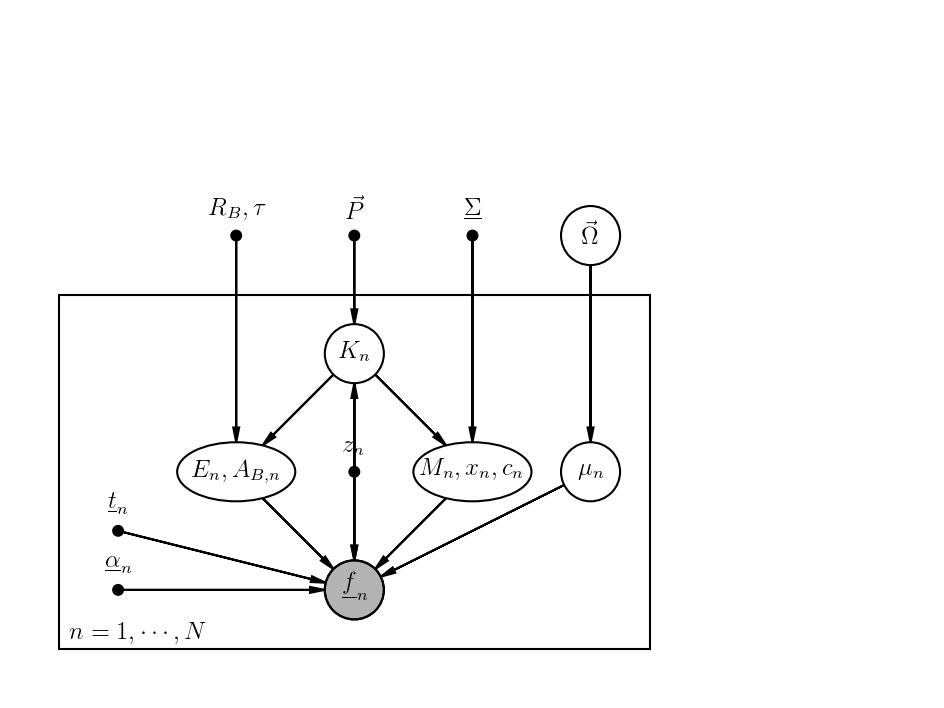
\includegraphics[width=0.5\textwidth]{sn-draft.png}
\caption{This directed acyclic graph represents the problem we wish to solve.  We would like to obtain the posterior over the cosmological parameters comprising $\vec{\Omega}$ given the data of observed photometry $\{\textul{f}_{n}\}_{N}$ (and the times of observation).  To do this, we must marginalize over the times of peak brightness (or times of supernovae initiations) $\{t_{n}\}_{N}$, the lightcurve fit parameters $\{M_{n},x_{n},c_{n}\}_{N}$, the dust and reddening parameters $\{E_{n},A_{B,n}\}_{N}$, the distance moduli $\{\mu_{n}\}_{N}$, the supernova types $\{K_{n}\}_{N}$, and the true photometry $\{\textul{f}_{0,n}\}_{N}$.  We take the following quantities as known constants: true redshifts $\{z_{n}\}_{N}$ and observing "nuisance" parameters $\{\textul{\alpha}_{n}\}_{N}$ as well as the parent distribution parameters $\textul{\Sigma}$ for the lightcurve fit parameters, $\vec{P}$ for the supernova type prevalences, $R_{B},\tau$ for the dust and reddening parameters, and $T$ (probably a uniform distribution) for the supernova times.}
\label{fig:pgm}
\end{center}
\end{figure}
%
%The model of Fig. \ref{fig:pgm} corresponds to the following equations for the posterior probability distribution $p(H|\{\textul{d}_{n}\}_{N})$.  
%
%\begin{align*}
%p(H|\{\textul{d}_{n}\}_{N}) &=\ p(\{\textul{d}_{n}\}_{N}|H)\frac{p(H)}{p(\{\textul{d}_{n}\}_{N})}\\
%&\ p(\{\textul{d}_{n}\}_{N}|H)p(H)\\
%&\propto\ \iint\ p(\{\textul{d}_{n}\}_{N}|H,D,S)\ p(H,D,S)\ dD\ dS\\
%&\propto\ \iint\ p(\{\textul{d}_{n}\}_{N}|H,D,S)\ p(H)\ p(D)\ p(S)\ dD\ dS\\
%&\propto\ \iint\ \left[\prod_{n=1}^{N}\ p(\textul{d}_{n}|H,D,S)\right]\ p(H)\ p(D)\ p(S)\ \ dD\ dS\\
%&\propto\ \iint\ \left[\prod_{n=1}^{N}\ \int\ p(\textul{d}_{n}|\textul{\ell}_{n},\vec{f},\textul{t})\ p(\textul{\ell}_{n}|H,D,S)\ d\textul{\ell}_{n}\right]\ p(H)\ p(D)\ p(S)\ dD\ dS\\
%&\propto\ \iint\ \left[\prod_{n=1}^{N}\ \int\ p(\textul{d}_{n}|\textul{\ell}_{n},\vec{f},\textul{t})\ \left[\iiint\ p(\textul{\ell}_{n}|z_{n},r_{n},s_{n})\ p(z_{n},r_{n},s_{n}|H,D,S)\ dz_{n}\ dr_{n}\ ds_{n}\right]\ d\textul{\ell}_{n}\right]\\
%&\indent p(H)\ p(D)\ p(S)\ dD\ dS\\
%&\propto\ \iint\ \left[\prod_{n=1}^{N}\ \int\ p(\textul{d}_{n}|\textul{\ell}_{n},\vec{f},\textul{t})\ \left[\iiint\ p(\textul{\ell}_{n}|z_{n},r_{n},s_{n})\ p(z_{n}|H)\ p(r_{n}|D)\ p(s_{n}|S)\ dz_{n}\ dr_{n}\ ds_{n}\right]\ d\textul{\ell}_{n}\right]\\
%&\indent p(H)\ p(D)\ p(S)\ dD\ dS
%\end{align*}

\section{Classification Methods}

There are a number of potentially probabilistic supernova type classification methods in the literature, each of which will be reviewed here.  Many of these are compared in \citet{Kessler10}, and they are summarized in Tab. \ref{tab:comp}.  

\begin{tabular}{ccccc}
\label{tab:comp}
References&Inputs&Outputs&Availability&Applications\\
\citet{Kuznetsova06}&&&&\\
\citet{Poznanski06}&&&&\\
\citet{Rodney09, Rodney10}&&&&\\
\citet{Sako11}&&&&\citet{Sako14}\\
\end{tabular}

\subsection{First(?) Bayesian Approach}

\citet{Kuznetsova06} is the first paper I can find on a probabilistic classifier, but it takes data of the form of a single band, multi-epoch lightcurve and a deterministic redshift.  This template-based method assumes the templates completely span the space of possible lightcurves and takes a $\chi^{2}$ likelihood model for the parameters of the fit between template and data.  They plug this into Bayes' Rule and integrate over types in the likelihood term (with a prior on type prevalence) to obtain a posterior.  They also assume a flat prior over prevalence of each type, which heavily biases their results whether or not they realize this.

\subsection{SN-ABC}

\citet{Poznanski06} is a probabilistic classifier that assigns supernovae a maximum likelihood type (Ia or core-collapse) based on single epoch, multi-band photometry and a photometric, spectroscopic, or probabilistic redshift for the host galaxy.  The likelihood of data given each of a grid of models for each type is calculated (assuming a $\chi^{2}$ form), and then the grid information (redshift, extinction, and epoch) is integrated out.  The evidence ratio (the ratio of the integral of likelihood over marginalized parameters and the sum of those integrals for all types) is declared to be a probability of a supernova being of that type, and the maximum probability type is assigned to the supernova.

\subsection{SOFT}

\citet{Rodney09, Rodney10} present the BATM (which seems to have math that is consistent with but distinct from BEAMS) and SOFT approaches to probabilistic classification.  I'm unsure if this approach is appropriate because we believe the supernovae actually do belong to discrete, deterministic sets.  However, when applied to the problem we wish to solve, it appears to perform quite well.

BATM employs a Gaussian likelihood to relate a model lightcurve (from a template set based on observed supernovae of each type) to data and Bayesian model comparison techniques to obtain the classification probabilities for each supernova.  This works when the template lightcurves are discrete, the template set spans the space of lightcurves represented in the data, and there are no duplicates in the template set.  

SOFT is proposed for when the above assumptions are violated.  In particular, a discrete template set cannot span the continuous space of lightcurves.  The authors introduce fuzzy set theory in which every supernova has a membership grade corresponding to each model spectrum and permitting partial membership in multiple classes.  They do, however, evaluate a point estimate classification based on membership grades.

\subsection{PSNID}

Photometric SN Identification (PSNID) \citep{Sako11} outputs the MAP type based on a $\chi^{2}$ fit, without providing the probabilities for each type, much like \citet{Poznanski06} but permitting multiple non-Ia types.  It also permits specification of the rates for each template type and provision of arbitrary templates, as well as an MCMC exploration of $\chi^{2}$ as opposed to a traditional grid search.  PSNID is incorporated into SNANA and is extremely similar to SN-ABC in its overall approach.  The differences are more freedom in the number of classes and the variables that are free in the $\chi^{2}$ fits.

\subsection{Machine Learning}

Nearest neighbor methods have been applied by \citet{Sako14} in an extension of PSNID.

Tree-based methods have been explored recently in the literature \citep{Richards11, Sako14, Lochner16, Moller16}.  While they do in theory produce probabilities over classes, they have always been used only to make deterministic classifications thus far.  \citet{Sako14} employs a kd-tree nearest neighbor algorithm.

Other machine learning approaches have also been investigated.  \citet{Varughese15} uses adaptive wavelets.  \citet{Karpenka12, Charnock16} use recurrent neural networks.  \citet{Lochner16} compares several of these approaches.

%\acknowledgments

%\appendix

\bibliography{references-sne1a}

\end{document}